\chapter{Objetivos}
\label{cap:capitulo2}

En este capítulo se describen los objetivos de este proyecto, así como los requerimientos, el método seguido y la estructura del mismo.\\

\section{Descripción del problema}
\label{sec:descripcion_problema}

Los drones son una herramienta tremendamente versátil, ya que permiten solventar los inconvenientes orográficos de forma sencilla, y pueden ser provistos de múltiples sensores, lo que incrementa su adaptabilidad para solucionar un gran abanico de retos ingenieriles.\\

Por tanto, el objetivo principal de este \ac{TFG} es desarrollar un comportamiento autónomo basado en \ac{RL}, sobre un dron para detectar y localizar el origen de una señal \ac{RF}. Esto puede ser especialmente útil en labores de rastreo e identificación de objetivos, tales como en casos de escenarios catastróficos donde se deben localizar personas perdidas o de rastreo de señales en entornos de interior.\\

Para ello, se establecen los siguientes subobjetivos:

\begin{enumerate}
	\item Desarrollo de una aplicación, enfocada a teleoperar un \ac{UAV}, empleando herramientas de simulación y visualización.
	\item Implementación de un modelo de propagación de señales, que nos ayude en el análisis para entornos simulados.
	\item Desarrollo de un comportamiento autónomo capaz de detectar y navegar hacia la fuente de una señal \ac{RF}.
	\item Comparativa frente a los algoritmos navegación tradicionales.
	\item Desarrollo de un comportamiento autónomo para que el dron navegue y detecte el transmisor, en un escenario dinámico.
\end{enumerate}

\section{Requisitos}
\label{sec:requisitos}

Las especificaciones que se deben cumplir son las siguientes:

\begin{enumerate}
	\item El modelo de propagación de señal debe basarse en el modelo de Friis.
	\item Se debe usar \ac{ROS} como middleware robótico y Gazebo como herramienta de simulación.
	\item Se debe seleccionar el algoritmo que navegue de forma más eficiente en cuanto a tiempo, movimientos y acciones hacia puntos con mayor potencia de señal.
	\item Se debe seleccionar el algoritmo más seguro en cuanto a salvaguardar la integridad del dispositivo y sus alrededores.
\end{enumerate}

\section{Metodología}
\label{sec:metodologia}

Este trabajo, comenzó oficialmente en Septiembre de 2022, aunqué se pusieran en común las ideas a principios del verano, y se concluye a finales de Septiembre de 2023.\\ 

La metodología para llevarlo a cabo fue la siguiente:

\begin{enumerate}
	\item Reunión de control semanal o cada dos semanas vía Teams con el tutor, donde se realizaba una valoración del estado del proyecto y se establecían los futuros puntos a seguir.
	\item Uso de la metodología Kanban, que es una metodología visual para gestionar y optimizar el flujo de trabajo a través de tarjetas y límites de trabajo en curso.
	\item Empleo de la plataforma Github, a fin de establecer un repositorio común\footnote[1]{\url{https://github.com/RoboticsLabURJC/2022-tfg-cristian-sanchez}}, como sistema de control de versiones y de almacenamiento de backups.
	\item Desarrollo de un blog donde se describe el estado del proyecto\footnote[2]{\url{https://roboticslaburjc.github.io/2022-tfg-cristian-sanchez/}}.
\end{enumerate}

\begin{figure} [H]
	\begin{center}
	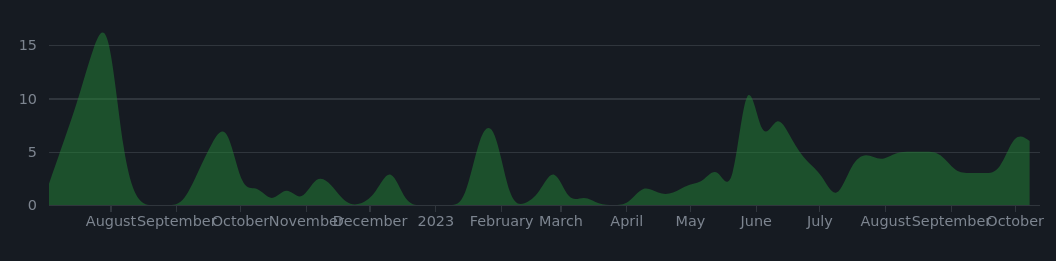
\includegraphics[height=3cm]{imagenes/cap2/1_insights.png}
	\end{center}
	\caption[Insights Github por meses \ac{TFG}]{Insights Github por meses \ac{TFG}}
	\label{fig:insights}
\end{figure}

\section{Plan de trabajo}
\label{sec:plantrabajo}

Para concluir este capítulo, los pasos seguidos han sido:

\begin{enumerate}
	\item Etapa inicial, donde tras establecer los objetivos del proyecto, se empezó por investigar el estado del arte del uso de drones para aplicaciones robóticas.
	\item Los primeros pasos en el \ac{TFG} se centrarón realizar una aplicación para teleoperar a un dron.
	\item El siguiente punto se basó en el estudio y comprensión de las señales \ac{RF} dentro del espectro de radiofrecuencia, con el fin de desarrollar un modelo de propagación.
	\item Posteriormente, se desarrollaron diversas soluciones encargadas de resolver el problema de detectar y navegar hacia una señal.
	\item A continuación, se realizó una fase de pruebas y extracción de información sobre la que se realizaron diversas comparativas.
	\item Cerrando la fase de desarrollo, lo último fue implementar soluciones sobre escenarios más realistas que incluían obstáculos.
	\item Finalmente, se realizó la redacción de la memoria.
\end{enumerate} 